% !Mode:: "TeX:UTF-8"
\documentclass[11pt]{article}
\usepackage[letterpaper, margin = 2cm]{geometry}
\usepackage{microtype}
\usepackage{parskip}
\usepackage{amssymb}
\usepackage{amsmath}
\usepackage{multicol}
\usepackage{graphicx}
\usepackage{booktabs}
\usepackage{caption}
\usepackage{subcaption}
\usepackage{float}
\usepackage[style=ieee]{biblatex}
\usepackage[bookmarks, unicode]{hyperref}

\addbibresource{heat_flux.bib}

\title{Heat Flux}
\author{Josh Kraan}
\date{\today}

\begin{document}

\maketitle

\section{Introduction}
In this document a new procedure to calculate heat flux using Cantera is detailed. The Feynman ``Downsized 2'' outputs are used for all example calculations.

The work here will make future heat flux calculations much easier. The effects of varying engine parameters can easily be seen without requiring the intermediate step of running them through NASA's CEA program, which is easy to misuse.

The heat flux calculated here will be used to look at the feasability of regenerative cooling, and could also be integrated with film cooling calulations being done by other team members.

\section{Gas Properties}

Combustion gas properties are commonly calculated using NASA's Chemical Equilibrium with Applications (CEA)~\cite{gorden_computer_1996} program, however this FORTRAN program is difficult to work with. Instead the combustion gas properties were calculated using Cantera as described by Youngblood~\cite{youngblood_design_2015}.

Species included in the chemical equilibrium calculations were based off of those used in CEA and kerosene combustion models~\cite{wang_thermophysics_2001} as well as the availability of transport properties. The species that were included in this analysis are: RP-1, LOX, CO, CO2, H, H2, H2O, O, OH, and O2. RP-1 and LOX were modeled with the same stoichiometry and heat of formation as used in CEA. Cantera requires transport parameters for all species, so RP-1 and LOX were assigned placeholder values with the understanding that equilibrium solutions contain essentially zero concentration of these species.

Thermodynamic properties and Lennard-Jones transport parameters were taken from a high-temperature version of the GRI MECH 3.0 combustion mechanism~\cite{smith_gri-mech_????} included with Cantera that has been extended from an upper temperature of 3500K to 6000K using the NASA Glenn Coefficients~\cite{mcbride_nasa_2002}.

\subsection{Property Evaluation}

The procedure used to calculate the gas properties differs significantly from CEA. Instead of using a user-specified chamber pressure, the properties are calculated from engine geometry and flow rates.

The first step is the calculate the stagnation and throat properties, which are solved for together. At the throat of the engine, the following two conditions must be met~\cite{martinez-sanchez_reacting_????}:
\begin{equation}\label{cond:mach}
  v = a
\end{equation}%
\begin{equation}\label{cond:enthalpy}
  h_0 = h + \frac{v^2}{2}
\end{equation}

The velocity and sound speed are calculated as follows:
\begin{equation}
  v = \frac{\dot{m}}{A \rho}
\end{equation}%
\begin{equation}
  a = \sqrt{\left(\frac{\partial p}{\partial \rho}\right)_s}
\end{equation}

The partial derivative required to calculate the sounds speed is evaluated by perturbing the pressure at constant entropy~\cite{_cantera_????}. If equilibrium expansion is used, the perturbed gas is equilibrated.

For a given stagnation pressure, the stagnation gas properties can be fully calculated as described by Youngblood. The throat conditions can then be solved for by varying the throat pressure isentropically until condition~\ref{cond:mach} is met. If condition~\ref{cond:enthalpy} is met, the stagnation pressure is correct, if not, another stagnation pressure must be guessed. Two root finders were used to solve for the chamber and throat properties in this manner.

With the stagnation enthalpy known, the conditions at all other points of the engine can be solved for by varying the pressure isentropically until condition~\ref{cond:enthalpy} is met. Both subsonic and supersonic solutions exist; specific solutions are forced by using the throat pressure to limit the solution range.


\subsection{Frozen Boundary Layer Chemistry}

CEA calculates ``frozen'' and ``equilibrium'' values for specific heat and thermal conductivity. Equilibrium values are taken to be the sum of the frozen value and a reaction term that accounts for chemical reactions occurring in the boundary layer. Equilibrium values for both are several times higher than frozen, and using the equilibrium values gives a calculated heat flux approximately 4.5 times higher (based on the Bartz equation).

Bartz~\cite[Page 46]{bartz_turbulent_1965} discusses chemical reactions occurring in rocket engine boundary layers and the resulting increase in heat transfer. When dissociated species such as O, H, and OH are present in the free stream, they can cool against combustion walls and recombine exothermically in the boundary layer. Bartz notes that this effect would likely be maximum for a hydrogen and oxygen rocket at 100\% combustion efficiency, yet the increase in heat flux over a frozen layer is shown to be only 32\% and rapidly decreases with reduced combustion efficiency.

The presence of dissociated species is not insignificant for this engine, as can be seen in Figure~\ref{fig:dissociated}. It is unclear why equilibrium values calculated by CEA are so high and reproducing them is difficult, so based off of the Bartz information the boundary layer was considered to be chemically frozen.

\begin{figure}[H]
  \centering
  \begin{subfigure}{.5\textwidth}
    \centering
    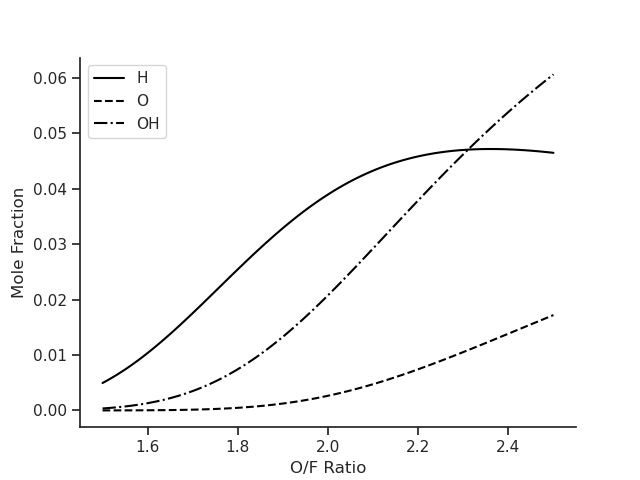
\includegraphics[width=\linewidth]{dissociated-chamber.png}
    \caption{Chamber}
  \end{subfigure}%
  \begin{subfigure}{.5\textwidth}
    \centering
    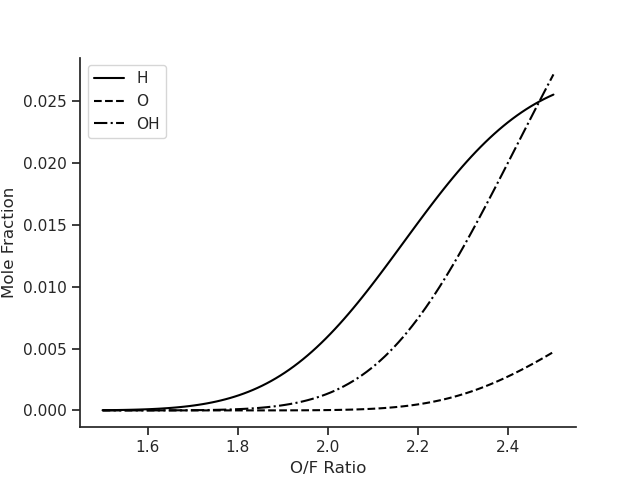
\includegraphics[width=\linewidth]{dissociated-nozzle.png}
    \caption{Nozzle}
  \end{subfigure}
  \caption{Dissociated species with equilibrium expansion, OF = 2.29.}
  \label{fig:dissociated}
\end{figure}

\subsection{Frozen Contraction and Expansion}

Through the contraction and expansion of the engine, combustion gas can be considered to either be in equilibrium (mole fractions change along length of engine) or the composition could be frozen. Both methods were implemented, but this was found to make little difference to heat flux calculations.

%TODO look into more

\subsection{Property Comparison}


\begin{table}[H]
  \centering
  \caption{Cantera and CEA comparison, equilibrium expansion, OF = 2.29.}
  \begin{tabular}{l c c c c c c}
    \toprule
    & \multicolumn{2}{c}{Stagnation} & \multicolumn{2}{c}{Throat} & \multicolumn{2}{c}{Exit} \\
    \cmidrule(lr){2-3} \cmidrule(lr){4-5} \cmidrule(lr){6-7}
    & Cantera & CEA Diff. & Cantera & CEA Diff. & Cantera & CEA Diff. \\
    \midrule
    P ($10^5$ Pa) & 8.3785 & N/A & 4.8249 & $0.37\%$ & 0.99181 & $0.01\%$ \\
    T (K) & 3314.8 & $-0.09\%$ & 3151.2 & $-0.06\%$ & 2697.0 & $-0.09\%$ \\
    $C_p$ ($10^3$ J/kg/K) & 2.0771 & $-0.05\%$ & 2.0675 & $-0.07\%$ & 2.0325 & $0.09\%$ \\
    $\rho$ ($10^{-1}$ kg/m$^3$) & 6.6174 & $0.06\%$ & 4.0651 & $0.39\%$ & 1.0093 & $0.07\%$\\
    $\mu$ ($10^{-5}$ Pa s) & 9.4775 & $8.06\%$ & 9.1404 & $8.21\%$ & 8.1726 & $8.64\%$ \\
    $k$ ($10^{-1}$ W/m/K) & 3.5689 & $-3.79\%$ & 3.3898 & $-3.55\%$ & 2.8982 & $-2.86\%$\\
    \bottomrule
  \end{tabular}
\end{table}

All major species were found to have less than 1\% difference in mole fractions between Cantera and CEA throughout the engine. Stagnation thermodynamic properties match very well, which is expected as GRI MECH uses the same thermodynamic data as CEA. Transport properties are consistently different; the empirical fits used by CEA are likely more accurate than the Lennard-Jones model used here, however the difference in calculated heat flux was found to be small.

\section{Heat Transfer Correlations}\label{sec:heat_transfer}

It appears to be accepted to use the difference between the adiabatic wall temperature and the wall temperature as the driving potential for heat flux~\cite{huang_modern_1992, bartz_turbulent_1965, grisson_liquid_1991}, so that was adopted here as well. The adiabatic wall temperature is given by:

\begin{equation}
    T_{aw} = T + r(T_0 - T)
\end{equation}

The recovery factor $r$ is commonly given as:

\begin{equation}
    r = (Pr)^{1/3}
\end{equation}

The gas wall temperature was taken to be a constant value of 300K, as would be the case on engine startup. The influence of the gas wall temperature is discussed in Section~\ref{sec:wall_temp}.

When property evaluation at temperatures other than the free stream temperature is required, the gas temperature was changed in Cantera while keeping the pressure constant.

\subsection{Bartz}

The Bartz equation is commonly used for calculating rocket engine heat flux. The following form is common:

\begin{equation}
    \label{equation:bartz}
    \begin{split}
         h_g = \left[ \frac{0.026}{D_t^{0.2}} \left( \frac{\mu^{0.2} c_p}{{Pr}^{0.6}} \right)_{0} \left( \frac{p_0}{c^*} \right)^{0.8} \left( \frac{D_t}{R_c} \right)^{0.1} \right] \left( \frac{A_t}{A} \right)^{0.9} \sigma \\
         \sigma = \frac{1}{\left[ \frac{1}{2} \left( \frac{T_{w}}{T_0} \right) \left( 1 + \frac{\gamma - 1}{2} M^2 \right) + \frac{1}{2}\right]^{0.8-m/5} \left[ 1 + \frac{\gamma - 1}{2} M^2 \right]^{m/5}}
    \end{split}
\end{equation}

Here $m$ is the exponent of the temperature dependence of viscosity, and it is commonly taken to be 0.6. The $\sigma$ term accounts for property variation in the boundary layer and along the length of the engine.

If the equation is rearranged into nondimensional parameters the fact that it is a modified version of the Dittus-Boelter equation is more clear:

\begin{equation}\label{equation:bartz1}
  Nu_{t} = 0.026 Re_{t}^{0.8} Pr^{0.4} \left( \frac{D_t}{R_c} \right)^{0.1} \left( \frac{A_t}{A} \right)^{0.9} \sigma
\end{equation}

Here all gas properties are evaluated at stagnation and the throat diameter is the characteristic dimension.

Another form given by Bartz also uses the stagnation gas properties but the characteristic dimension is the local diameter. It has a boundary layer property variation term that uses the gas viscosity and density at the arithmetic mean of the free stream and wall temperatures:

\begin{equation}\label{eqn:bartz_free}
  Nu_{D} = 0.026 Re_{D}^{0.8} Pr^{0.4} \left( \frac{D_t}{R_c} \right)^{0.1} \left[ \left( \frac{\rho_{am}}{\rho} \right)^{0.8} \left(\frac{\mu_{am}}{\mu} \right)^{0.2}\right]
\end{equation}

Three forms of the Bartz equation are graphed. The version with a property variation term (Equations~\ref{equation:bartz}~\&~\ref{equation:bartz1}) is shown based off of both purely CEA data with $m=0.6$ and Cantera data where $m=0.75$ was found to better fit the temperature dependence of the gas viscosity. The free stream version of Bartz (Equation~\ref{eqn:bartz_free}) is also shown.

\subsection{Dittus-Boelter}

The unmodified Dittus-Boelter equation the Bartz equation is based on is given by:

\begin{equation}
  Nu_{D} = 0.023 Re_{D}^{0.8} Pr^{0.4}
\end{equation}

The Dittus-Boelter equation is known to be ill-suited to modeling flows with large property variations in the boundary layer~\cite{bergman_fundamentals_2017}. A proposed solution is to evaluate all properties at the arithmetic mean of the free stream and wall temperatures~\cite{bartz_turbulent_1965, grisson_liquid_1991}.

\subsection{Sieder-Tate}

When continuing with the theme of applying simple pipe-flow correlations to rocket engine heat transfer, the Sieder-Tate correlation seems relevant (as it is known for better modeling large property variations~\cite{bergman_fundamentals_2017}). All properties are evaluated at the free stream temperature except for $\mu_w$, which is evaluated at the wall temperature.

\begin{equation}
  Nu_{D} = 0.027 Re_{D}^{0.8} Pr^{1/3} \left( \frac{\mu}{\mu_w} \right)^{0.14}
\end{equation}

\section{Calculated Heat Flux}

The calculated heat flux using the methods described in Section~\ref{sec:heat_transfer} is shown in Figure~\ref{fig:heat_flux}.

\begin{figure}[H]
  \centering
  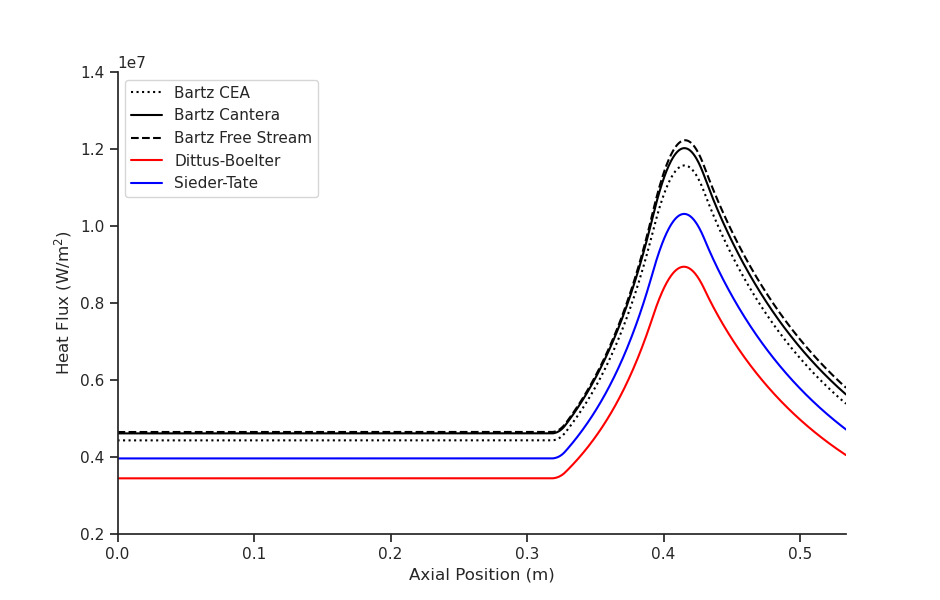
\includegraphics[width=\linewidth]{Heat_Flux.png}
  \caption{Calculated heat flux, OF=2.29.}
  \label{fig:heat_flux}
\end{figure}

The Bartz correlations all agree well and are within 5\% of each other. The heat flux calculated with CEA values is the lower than the two Cantera curves --- this is likely due to the difference in transport properties.

Despite directly applying the common Sieder-Tate equation to a rocket engine, it appears to match decently well with the Bartz values.

The largest difference was between the Dittus-Boelter and Bartz models, at 30\%. This was found to be because of the difference in constants (11\%), the throat curvature factor (10\%), and the breakdown of the assumption of constant Prandtl number and specific heat (9\%).

\section{Modifying Factors}

The free stream Bartz correlation (Equation~\ref{eqn:bartz_free}) is used to illustrate the following effects.

\subsection{OF Ratio}

The OF Ratio can be reduced by keeping the total mass flow rate the same, or by decreasing the fuel flow rate. The effects of both are shown in Figure~\ref{fig:of_ratio}.

\begin{figure}[H]
  \centering
  \begin{subfigure}{.5\textwidth}
    \centering
    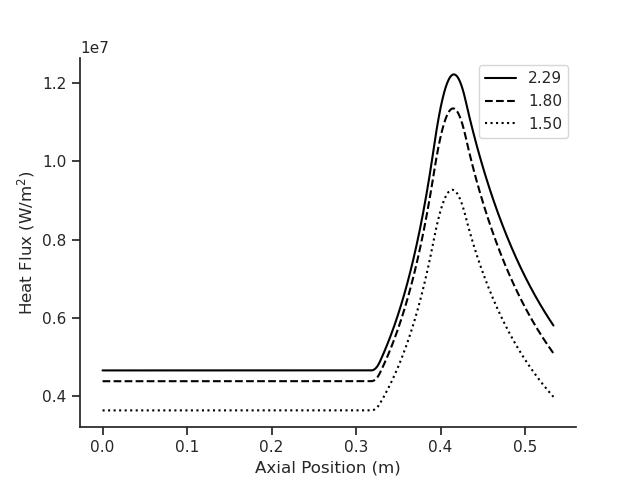
\includegraphics[width=\linewidth]{OF_Constant.png}
    \caption{Constant $\dot{m}$}
  \end{subfigure}%
  \begin{subfigure}{.5\textwidth}
    \centering
    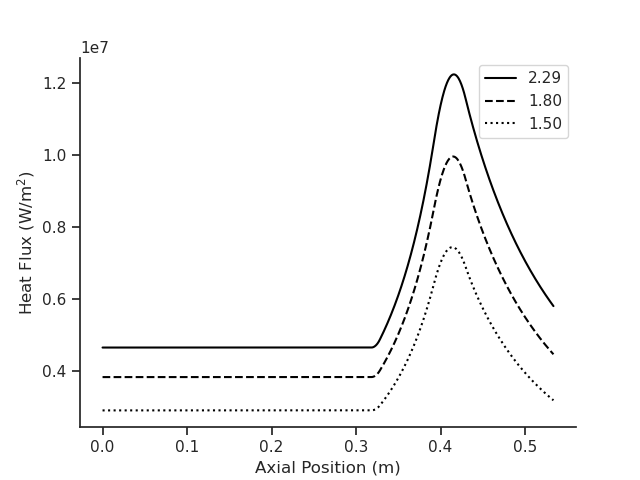
\includegraphics[width=\linewidth]{OF_Variable.png}
    \caption{Variable $\dot{m}$}
  \end{subfigure}
  \caption{Effects of OF ratio on heat flux.}
  \label{fig:of_ratio}
\end{figure}

Other factors not accounted for here may make this difference more dramatic. At higher OF ratios the presence of dissociated species is greater, which can increase heat flux, and at lower OF ratios the effect of carbon deposition on the walls is greater~\cite{cook_advanced_1980}.

\subsection{Frozen or Equilibrium Expansion}
As noted before, the effects of assuming equilibrium or frozen expansion were found to be minor, and are shown in Figure~\ref{fig:equilibrium}. Reality would be somewhere in between these two extremes.

\begin{figure}[H]
  \centering
  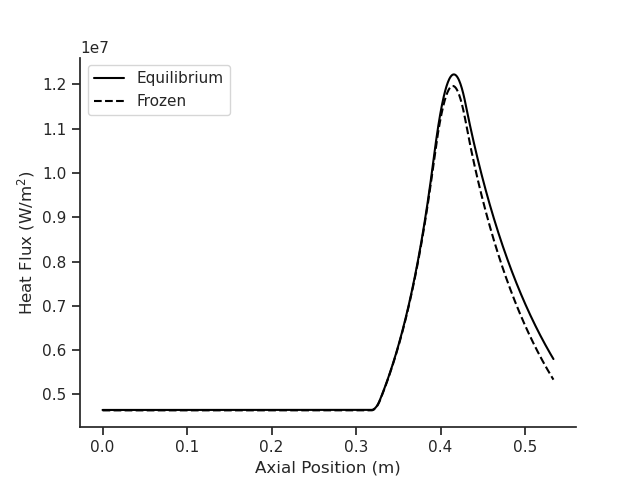
\includegraphics[width=0.5\linewidth]{Equilibrium_Frozen.png}
  \caption{Heat flux with frozen and equilibrium expansion, OF=2.29.}
  \label{fig:equilibrium}
\end{figure}

\subsection{Carbon Deposition}

Carbon deposition on combustion walls can significantly increase the thermal resistance and decrease the heat flux into the walls~\cite[Page 86]{huang_modern_1992}. This effect can also be increased by using fuel film cooling~\cite[Page 35]{campbell_thrust_1963}.

For calculating the heat flux with a carbon deposit, the deposit is assumed to be at the combustion gas temperature, and a modified heat transfer coefficient is calculated by using the thermal resistance of the deposit~\cite{huang_modern_1992}:
\begin{equation}
  h_{gc} = \frac{1}{\frac{1}{h_g} + R}
\end{equation}
Huang and Huzel give the thermal resistance of a carbon deposit for a 7 MPa engine as a function of area ratio, with values ranging from approximately $3.7 \times 10^{-4}$ m$^2$K/W to $6.8 \times 10^{-4}$ m$^2$K/W. The thermal resistance is lowest at the throat.

\subsection{Wall Temperature}\label{sec:wall_temp}

\subsection{Flow Recirculation}

The recirculation zones that cause the famous combustion stability of pintle injectors can also cause higher chamber heat flux than predicted, as the combustion gas velocity near the wall can be much larger than the average cross-sectional velocity~\cite[Page 81]{bartz_turbulent_1965}.

A (very) simple estimate of this effect can be found by assuming that the combustion gas in the inner half of the radius flows towards the injector at the same velocity as the outer half of the radius, which flows towards the nozzle. It can be shown that this velocity must be twice the cross sectionally averaged velocity. Based off of the correlations in Section~\ref{sec:heat_transfer}, this would increase the heat flux by $74\%$.

Bartz presents data for an Enzian injector, which features similar recirculation. The measured chamber heat flux is nearly $100\%$ higher than predicted --- surprisingly close to the crude estimate done here.

\subsection{Combustion Efficiency}
The previous results have all assumed perfect combustion performance. If the combustion efficiency is reduced, the chamber pressure and temperature would change, as well as species mole fractions.

From the correlations in Section~\ref{sec:heat_transfer} it can be seen that the heat transfer coefficient is proportional to the mass flux to the 0.8 power:
\begin{equation}
  h_g \propto \left(\frac{\dot{m}}{A}\right)^{0.8}
\end{equation}
The throat mass flux is more or less proportional to the chamber pressure:
\begin{equation}
  \frac{\dot{m}}{A_t}  = p_0 \sqrt{\frac{\gamma [2 / (\gamma + 1)]^{\frac{\gamma + 1}{\gamma - 1}}}{R_{gas} T_o}}
\end{equation}
This leads to the oft-cited result that the throat heat flux is proportional to the chamber pressure to the 0.8 power. However, in the case of inefficient combustion, the chamber pressure would decrease, but the mass flux would stay the same. The largest reduction in heat flux would most likely come from the reduction in the combustion gas temperature.

The form of equation~\ref{equation:bartz} is useful when looking at the influence of parameter changes. The gas specific heat and Prandtl number are relatively constant over a wide temperature range. The gas viscosity varies significantly, however it is only to power of 0.2. This indicates it would likely take a large reduction in combustion performance to produce a significantly lower heat flux than calculations assuming perfect combustion.

\section{Conclusion}

Pintle recirculation zones

Film cooling

\printbibliography



\end{document}
